\subsection{UDP / TCP}
To analyse the power consumption while sending data to an client we prepared a 
experiment where we send data in a loop to a client over TCP and UDP.\\

\subsubsection{Experimental setup}
To measure the power consumption we had to extend the setup from Fig.\ref{fig:experiment_setup}.
Because the ESP8266 verified its connection to the access point while idle.
To distinguish between the verifying of the connection and the transmitting of
data we log the transmitting process.
In order to obtain only the meaningful parts of the measurements,
we have prepared a trigger via the I/O pins. While the ESP is transmitting,
the PIN 2 goes high.
On the other side the microcontroller logs the lines with 1 when the pin 1 gets current.
\newline
\begin{figure}[h]
\centering
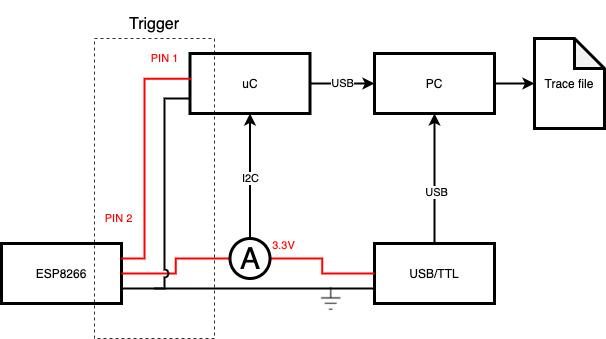
\includegraphics[width = 0.90 \linewidth]{fig/udp_tcp/experimental_setup_udp_tcp.png}
\caption{Setup to measure the current consumption while sending data with the ESP8266.}
\label{fig:experiment_udp_tcp}
\end{figure}
\subsubsection{TCP}
In order to analyze the power consumption when sending data via UDP,
we have prepared a function that transfers data from an ESP8266 to a PC via a WiFi connection.
Whithen we listens to an open port with netcat.
To study the power consumption of TCP,
we will send data to a client over TCP using the ESP8266WiFi library.
In our experiment we prepared random packets to disable the TCP chaching system.
We then processed 100 iterations of the function in Fig.\ref{fig:tcp_uml}
to geather enough values.
\begin{figure}[h]
\centering
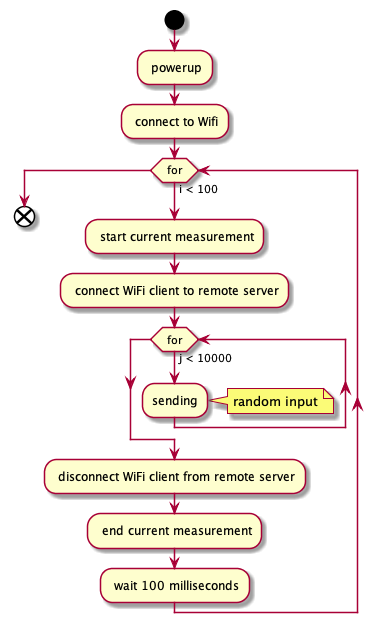
\includegraphics[width = 0.7 \linewidth]{fig/udp_tcp/tcp_uml.png}
\caption{process to sending data over TCP}
\label{fig:tcp_uml}
\end{figure}
\newline\newline
As expected, when we send data over TCP, we get a lot of different results.
This is because we have to wait for the recipient response to send the data.
\linebreak\linebreak
\begin{table}[htbp]
\begin{center}
\caption{Results TCP}
\label{tab:table1}
\renewcommand{\arraystretch}{1.8}
\begin{tabular}{l|c|r}
& \textbf{time [ms]} & \textbf{As}\\
\hline
count & 100 & 100\\
mean & 241.570 & 0.021031\\
std & 32.115403 & 0.002591\\
min & 193 & 0.016300\\
25\%  & 219 & 0.019175\\
50\% & 236 & 0.020600\\
75\%  & 257 & 0.022325\\
max & 396 & 0.032600\\
\end{tabular}
\end{center}
\end{table}
\linebreak
If we look at the results, we see that the current fluctuates a lot,
this is because TCP-buil-in system is monitoring the trasmitting 
and waiting for the recipient to receive the packet.\linebreak\linebreak
\begin{figure}[h!]
\centering
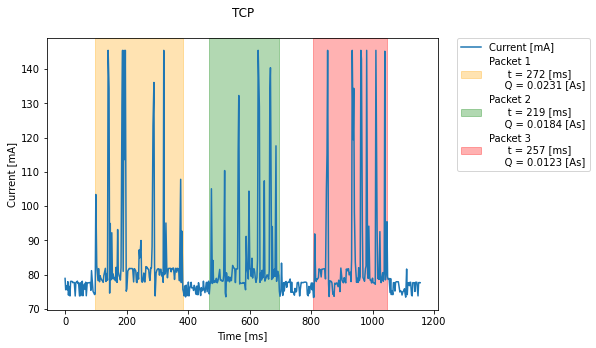
\includegraphics[width = 1 \linewidth]{fig/udp_tcp/tcp_s_m.png}
\caption{sending data over TCP}
\label{fig:tcp_s_m}
\end{figure}
\linebreak\linebreak
According these, also the elapsed time is 236$\pm$13.63\% ms
\linebreak
\begin{figure}[h!]
\centering
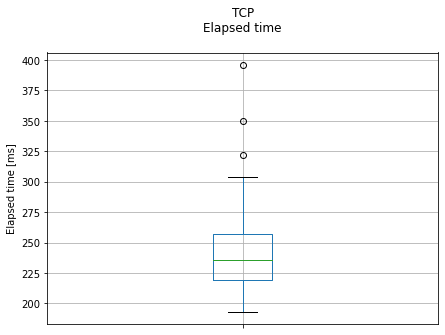
\includegraphics[width = 0.7 \linewidth]{fig/udp_tcp/tcp_boxplot_time.png}
\caption{elapsed time while sending over TCP}
\label{fig:tcp_boxplot_time}
\end{figure}
\linebreak
In addition, the power consumption is 0.0206$\pm$12.58\% As
\linebreak
\begin{figure}[h!]
\centering
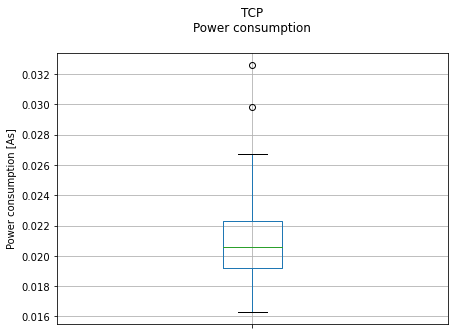
\includegraphics[width = 0.7 \linewidth]{fig/udp_tcp/tcp_boxplot_As.png}
\caption{ampere seconds while sending over TCP}
\label{fig:tcp_boxplot_As}
\end{figure}
\pagebreak
\subsubsection{UDP}
To analyse the power consumption while sending data over UDP we prepared a procedure which
transfer data from an ESP8266 to a generic notbook  via UDP from the WiFiUdp library.
In order to be able to compare with TCP, we create the process in Fig.\ref{fig:udp_uml}
\begin{figure}[h]
\centering
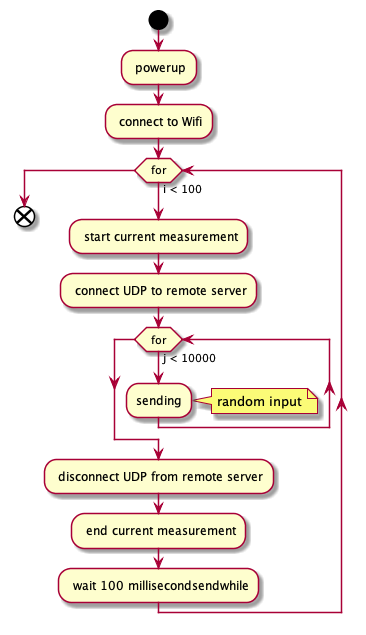
\includegraphics[width = 0.7 \linewidth]{fig/udp_tcp/udp_uml.png}
\caption{process to sending data over UDP}
\label{fig:udp_uml}
\end{figure}
\newline\newline
As expected, when we send data over UDP, we get more uniform values.
\linebreak\linebreak
\begin{table}[htbp]
\begin{center}
\caption{Results UDP}
\label{tab:table1}
\renewcommand{\arraystretch}{1.8}
\begin{tabular}{l|c|r}
& \textbf{time [ms]} & \textbf{As}\\
\hline
count & 100 & 100\\
mean & 95.970 & 0.009227\\
std & 1.058444 & 0.000581\\
min & 94 & 0.008200\\
25\% & 95 & 0.008800\\
50\% & 96 & 0.009100\\
75\% & 97 & 0.009600\\
max & 98 & 0.010900\\
\end{tabular}
\end{center}
\end{table}
\linebreak
If we look at the results, we see that the current is almost stable,
this is because UDP is not waiting for the recipient to receive the packet.
When it starts it sends the Packages simultaneously.\linebreak\linebreak
\begin{figure}[h!]
\centering
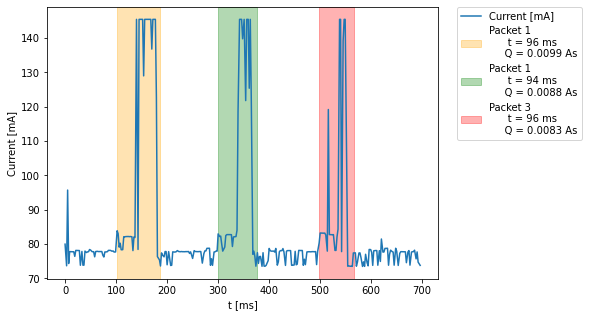
\includegraphics[width = 1 \linewidth]{fig/udp_tcp/udp_s_m.png}
\caption{sending data over UDP}
\label{fig:udp_s_m}
\end{figure}
\linebreak\linebreak
According these, also the elapsed time is 96$\pm$1.10\% ms
\linebreak
\begin{figure}[h!]
\centering
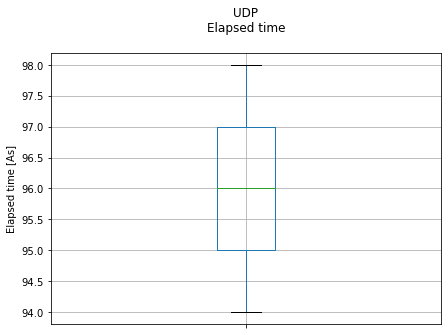
\includegraphics[width = 0.7 \linewidth]{fig/udp_tcp/udp_boxplot_time.png}
\caption{elapsed time while sending over UDP}
\label{fig:udp_boxplot_time}
\end{figure}
\linebreak
In addition, the power consumption is 0.0091$\pm$6.38\% As
\linebreak
\begin{figure}[h!]
\centering
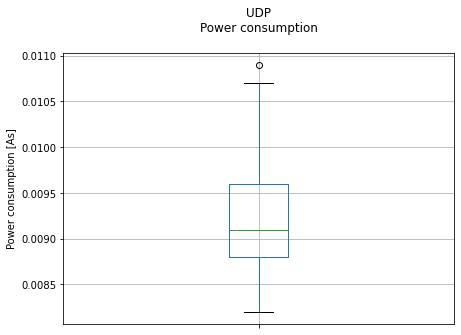
\includegraphics[width = 0.7 \linewidth]{fig/udp_tcp/udp_boxplot_As.png}
\caption{ampere seconds while sending over UDP}
\label{fig:udp_boxplot_As}
\end{figure}
\pagebreak